\documentclass{article}

\usepackage[inner=3cm,outer=3cm]{geometry} %left=4cm,right=2cm would be equivalent
\usepackage[utf8]{inputenc}
%\usepackage{hyperref}
%\usepackage{natbib}
\usepackage{amsmath}
\usepackage{parskip}
\usepackage{graphicx}
\usepackage{placeins}
\usepackage{float}
\usepackage{listings}
\usepackage{color}

\definecolor{dkgreen}{rgb}{0,0.6,0}
\definecolor{gray}{rgb}{0.5,0.5,0.5}
\definecolor{mauve}{rgb}{0.58,0,0.82}



\usepackage{xcolor}
\newcommand{\code}[1]{\texttt{#1}}
\author{octavia Crompton}

\begin{document}
\tableofcontents		
\section{ A two layer model}
\subsection{ Equations and assumptions}

The equations for the upper  and lower  canopies are:

\begin{equation}
    \frac{dG_u}{dt} =  r_{u} S^\beta G_u \big(1-\frac{G_u}{k_u}\big)
    \label{G_u}
\end{equation}

 \begin{equation}
    \frac{d G_l}{dt} = r_l S^\beta G_l \big(1-\frac{G_l}{k_l}\big) - \alpha G_u G_l,
        \label{G_l}
\end{equation}


where subscripts indicate the canopy level, $G$ is the biomass density, $r$ is the growth rate, $k$ is the carrying capacity, and $\alpha$ is a competition parameter, which effects the lower canopy only.

A vegetation growth limiting factor, $S^\beta$, slows the biomass growth rates as soil moisture decreases; this effect increases with increasing $\beta$.


Assume that fires occur with fixed return interval $\xi$  and severity $\phi_S$.

The biomass immediately before each fire  ($G_{u,max}$) and immediately after ($G_{uo}$) are related as:

\begin{equation}
    \frac{G_{u,max}}{G_{uo}} = \frac{1}{\phi_R}
\end{equation}

where $\phi_R$ is the proportion of biomass that remains after each fire.  Defining fire severity as $\phi_S = 1-\phi_R$:

\begin{equation}
    \frac{G_{u,max}}{G_{uo}} = 1 - \frac{1}{\phi_S}
\end{equation}


\subsection{  Analytic solution for the upper canopy}

Equation \ref{G_u}  is the logistic equation, and  has an analytic solution:
\begin{equation}
    G_u = \frac{k_u G_{uo}}{G_{uo} +(k_u-G_{uo}) e^{-r'_u t}}
    \label{logistic_solution}
\end{equation}

where  $G_{uo}$  is the initial biomass, and $r'_u =  r_u S^\beta  $  combines the growth rate and growth-limiting factor into an `effective` growth rate.

If time is measured as the time since the previous fire, then $G_u(t = 0) = G_{uo}$ and  $G_u(t = \xi) = G_{u,max}$  (once the system is in a dynamic steady state):

\begin{equation}
    \frac{G_{u,max}}{G_{uo}} = \frac{1}{\phi_R} =  \frac{k_u }{G_{uo} +(k_u-G_{uo}) e^{-r'_u \xi}}
\end{equation}

 Solving for $G_{uo}$:

\begin{equation}
  G_{uo} =  k_u \  \frac{\phi_R - e^{-r'_u \xi} }{1 - e^{-r'_u \xi}}
\end{equation}

Or, in terms of severity:

\begin{equation}
  G_{uo} =  k_u \   \frac{1- \phi_S - e^{-r'_u \xi} }{1 - e^{-r'_u \xi}}
  \label{G_uo}
\end{equation}

\subsection*{Mean upper canopy biomass}

Integrate Equation \ref{logistic_solution} to get average $G_u$:

\begin{equation*}
 \int_{G_{uo}}^{G_{u,max}} G_u dt =
 \int_{0}^\xi \frac{k_u G_{uo}}{G_{uo} +(k_u-G_{uo}) e^{- r'_u t}}dt
\end{equation*}

\begin{equation*}
 \quad  =\frac{k_u}{r'_u}\log \big(| G_{uo} - G_{uo} e^{r'_u\xi}  - k_u | \big)
  - \frac{k_u}{r'_u}\log \big(|  - k_u | \big),
\end{equation*}


which simplifies to:

\begin{equation*}
 \int_{G_{uo}}^{G_{u,max}} G_u dt =
 		 \frac{k_u}{r'_u}\log \big(1 + \frac{G_{uo}}{k_u}( e^{r'_u \xi}-1)\big)
\end{equation*}

Once the system is in dynamic equilibrium, the mean upper canopy biomass $\hat G_u$ is:

\begin{equation}
\hat{G}_u =
 		 \frac{k_u}{r'_u \xi}\log \bigg(1 + \frac{G_{uo}}{k_u}( e^{r'_u \xi}-1)\bigg)
\end{equation}

Substitute Equation  \ref{G_uo} and simplify:

\begin{equation}
\hat{G}_u =
 \frac{k_u}{r'_u \xi}\log \big(1 +   \frac{1- \phi_S - e^{-r'_u \xi} }{1 - e^{-r'_u \xi}} ( 1 - e^{-r'_u \xi})\big)
\end{equation}


\begin{equation}
\hat{G}_u =
  k_u \big( 1 + \frac{1}{r'_u \xi} \log(1-\phi_S) \big)
		\label{G_u_mean}
\end{equation}

     
\subsection{A modified logistic equation for the lower canopy}
    
    The equation for the lower canopy  is:
    
     \begin{equation}
        \frac{d G_l}{dt} = r_l S^\beta G_l \bigg(1-\frac{G_l}{k_l}\bigg) - \alpha G_u G_l
    \end{equation}
    
    Since we have an analytic solution for $\hat G_u$,  we can modify the logistic equation to solve for $\hat G_l$.
    Rewrite $G_l$  in logistic equation form:
    
      \begin{equation}
        \frac{d G_l}{dt} = r'_l \bigg(1-\frac{G_l}{k'_l}\bigg)
    \end{equation}

    where $r'_l = r_l S^\beta - \alpha \hat G_u$ and $k'_l  = k_l r'_l / r_l S^\beta$.
    
    The analytic solution for $G_{uo}$ (Equation \ref{G_uo}) can then be used to estimate $G_l$ after the fire:
    
    \begin{eqnarray}
      G_{lo} =  k'_l \   \frac{1- \phi_S - e^{-r'_l \xi} }{1 - e^{-r'_l \xi}}
    \end{eqnarray}
    
     Similarly, the analytic solution for the mean  biomass (Equation \ref{G_u_mean}) can be used to estimate  $\hat G_l$:
    
    \begin{equation}
    \hat{G}_l =
     		k'_l \bigg( 1 + \frac{1}{r'_l \xi} \log(1-\phi_S) \bigg)
    \label{hatG_l}
    \end{equation}
    
    Substitute $\hat G_u$ (Equation \ref{G_u_mean}) into $r'_l = r_l S^\beta - \alpha \hat G_u$ to get the modified growth rate:
    
    \begin{equation}
    r'_l= r_l S^\beta   - \alpha k_u \big( 1 + \frac{1}{r'_u \xi} \log(1-\phi_S) \big)
    \end{equation}
    
    And similarly for  $k'_l  = k_l r'_l / r_l S^\beta$:
    
    \begin{equation}
    k'_l= \frac{k_l}{r_l S^\beta } \bigg[  r_l S^\beta   - \alpha k_u \big( 1 + \frac{1}{r'_u \xi} \log(1-\phi_S) \big) \bigg]
    \end{equation}
    
    Which simplifies to:
    
    \begin{equation}
    k'_l=  k_l  \bigg[ 1 -  \frac{  \alpha k_u} {r_l S^\beta }\big( 1 + \frac{1}{r'_u \xi} \log(1-\phi_S) \big) \bigg]
    \end{equation}
  %%%%%%%%%%%%%%%%%%%%%%%%%%%%%%%%%%%%%%%%
  %%%%%%%%%%%%%%%% STABILITY %%%%%%%%%%%%%%%%%%
  %%%%%%%%%%%%%%%%%%%%%%%%%%%%%%%%%%%%%%%%
\section{Stability}

\subsection{Stability: conditions to sustain upper canopy biomass}

        Requiring that $\hat{G}_u >0$ in Equation \ref{G_u_mean} yields:
        
        \begin{equation}
        \phi_S < 1- e^{-r_u S^\beta \xi}
        \end{equation}
        
        In terms of return time:
        
        \begin{equation}
        \xi > - \frac{1}{r_u S^\beta}\log (1 - \phi_S)
        \end{equation}

	For lower growth rates, a longer return interval is needed to sustain biomass.  Increasing $\beta$ and/or decreasing $S$  lowers the effective upper canopy growth rate
	

% Figure
\begin{figure}[h]
 \centering
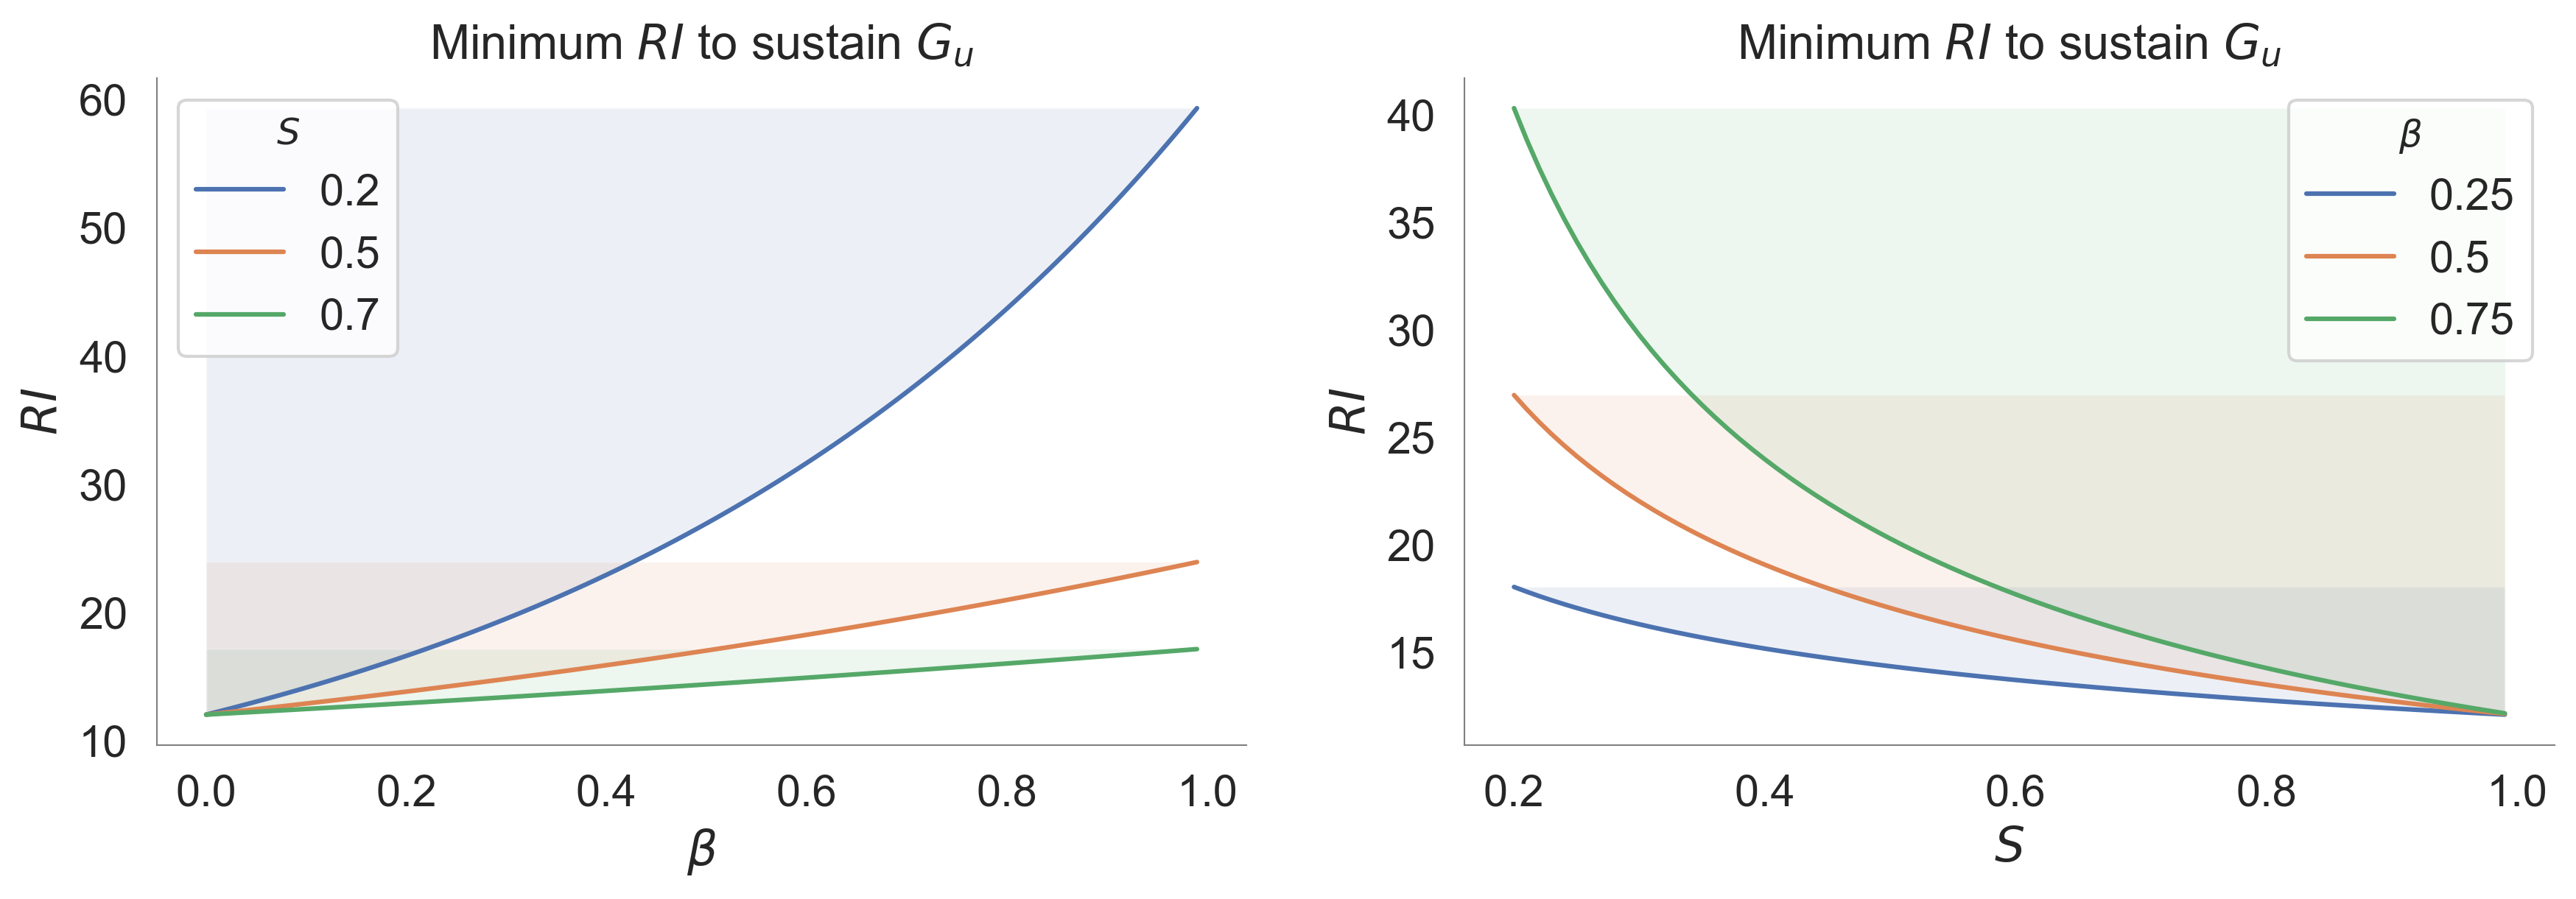
\includegraphics[width=33pc]{../fire_plots/stability_min_RI.png}
 \caption{ (a) }
 \label{fig:stability_min_RI.png}
 \end{figure}
 
         
If $\beta>0$, a longer return time is needed for lower soil moisture conditions:


Rearranging to find the minimum soil moisture to sustain the upper canopy:

\begin{equation}
S > \bigg( - \frac{1}{r_u \xi }\log (1 - \phi_S)\bigg)^{1/\beta}
\end{equation}

\begin{equation}
\hat{G}_u  =
    \begin{cases}
       k_u \big( 1 + \frac{1}{r'_u \xi} \log(1-\phi_S) \big)
	  & \text{if  } S > \big( - \frac{1}{r_u \xi }\log (1 - \phi_S)\big)^{1/\beta}
		\\[10pt]
      0 & \text{otherwise}
    \end{cases}
\end{equation}



\subsection{Stability: Relating return interval and severity for the upper canopy}
        
        Suppose $\hat G_u = \gamma k_u$, where $\gamma<1$. From  Equation \ref{G_u_mean}:
        
        \begin{equation}
        \gamma =  1 + \frac{1}{r'_u \xi} \log(1-\phi_S)
        \end{equation}
        
        \begin{equation}
        \xi = -\frac{1}{r'_u (1-\gamma) }\log(1-\phi_S)
        \end{equation}
        
        Rearranging for $\phi_S$:
        
        
        \begin{equation}
        \phi_S = 1- e^{-\xi r'_u (1-\gamma)}
        \label{max_severity}
        \end{equation}
        
        
        
 \begin{figure}[h]
 \centering
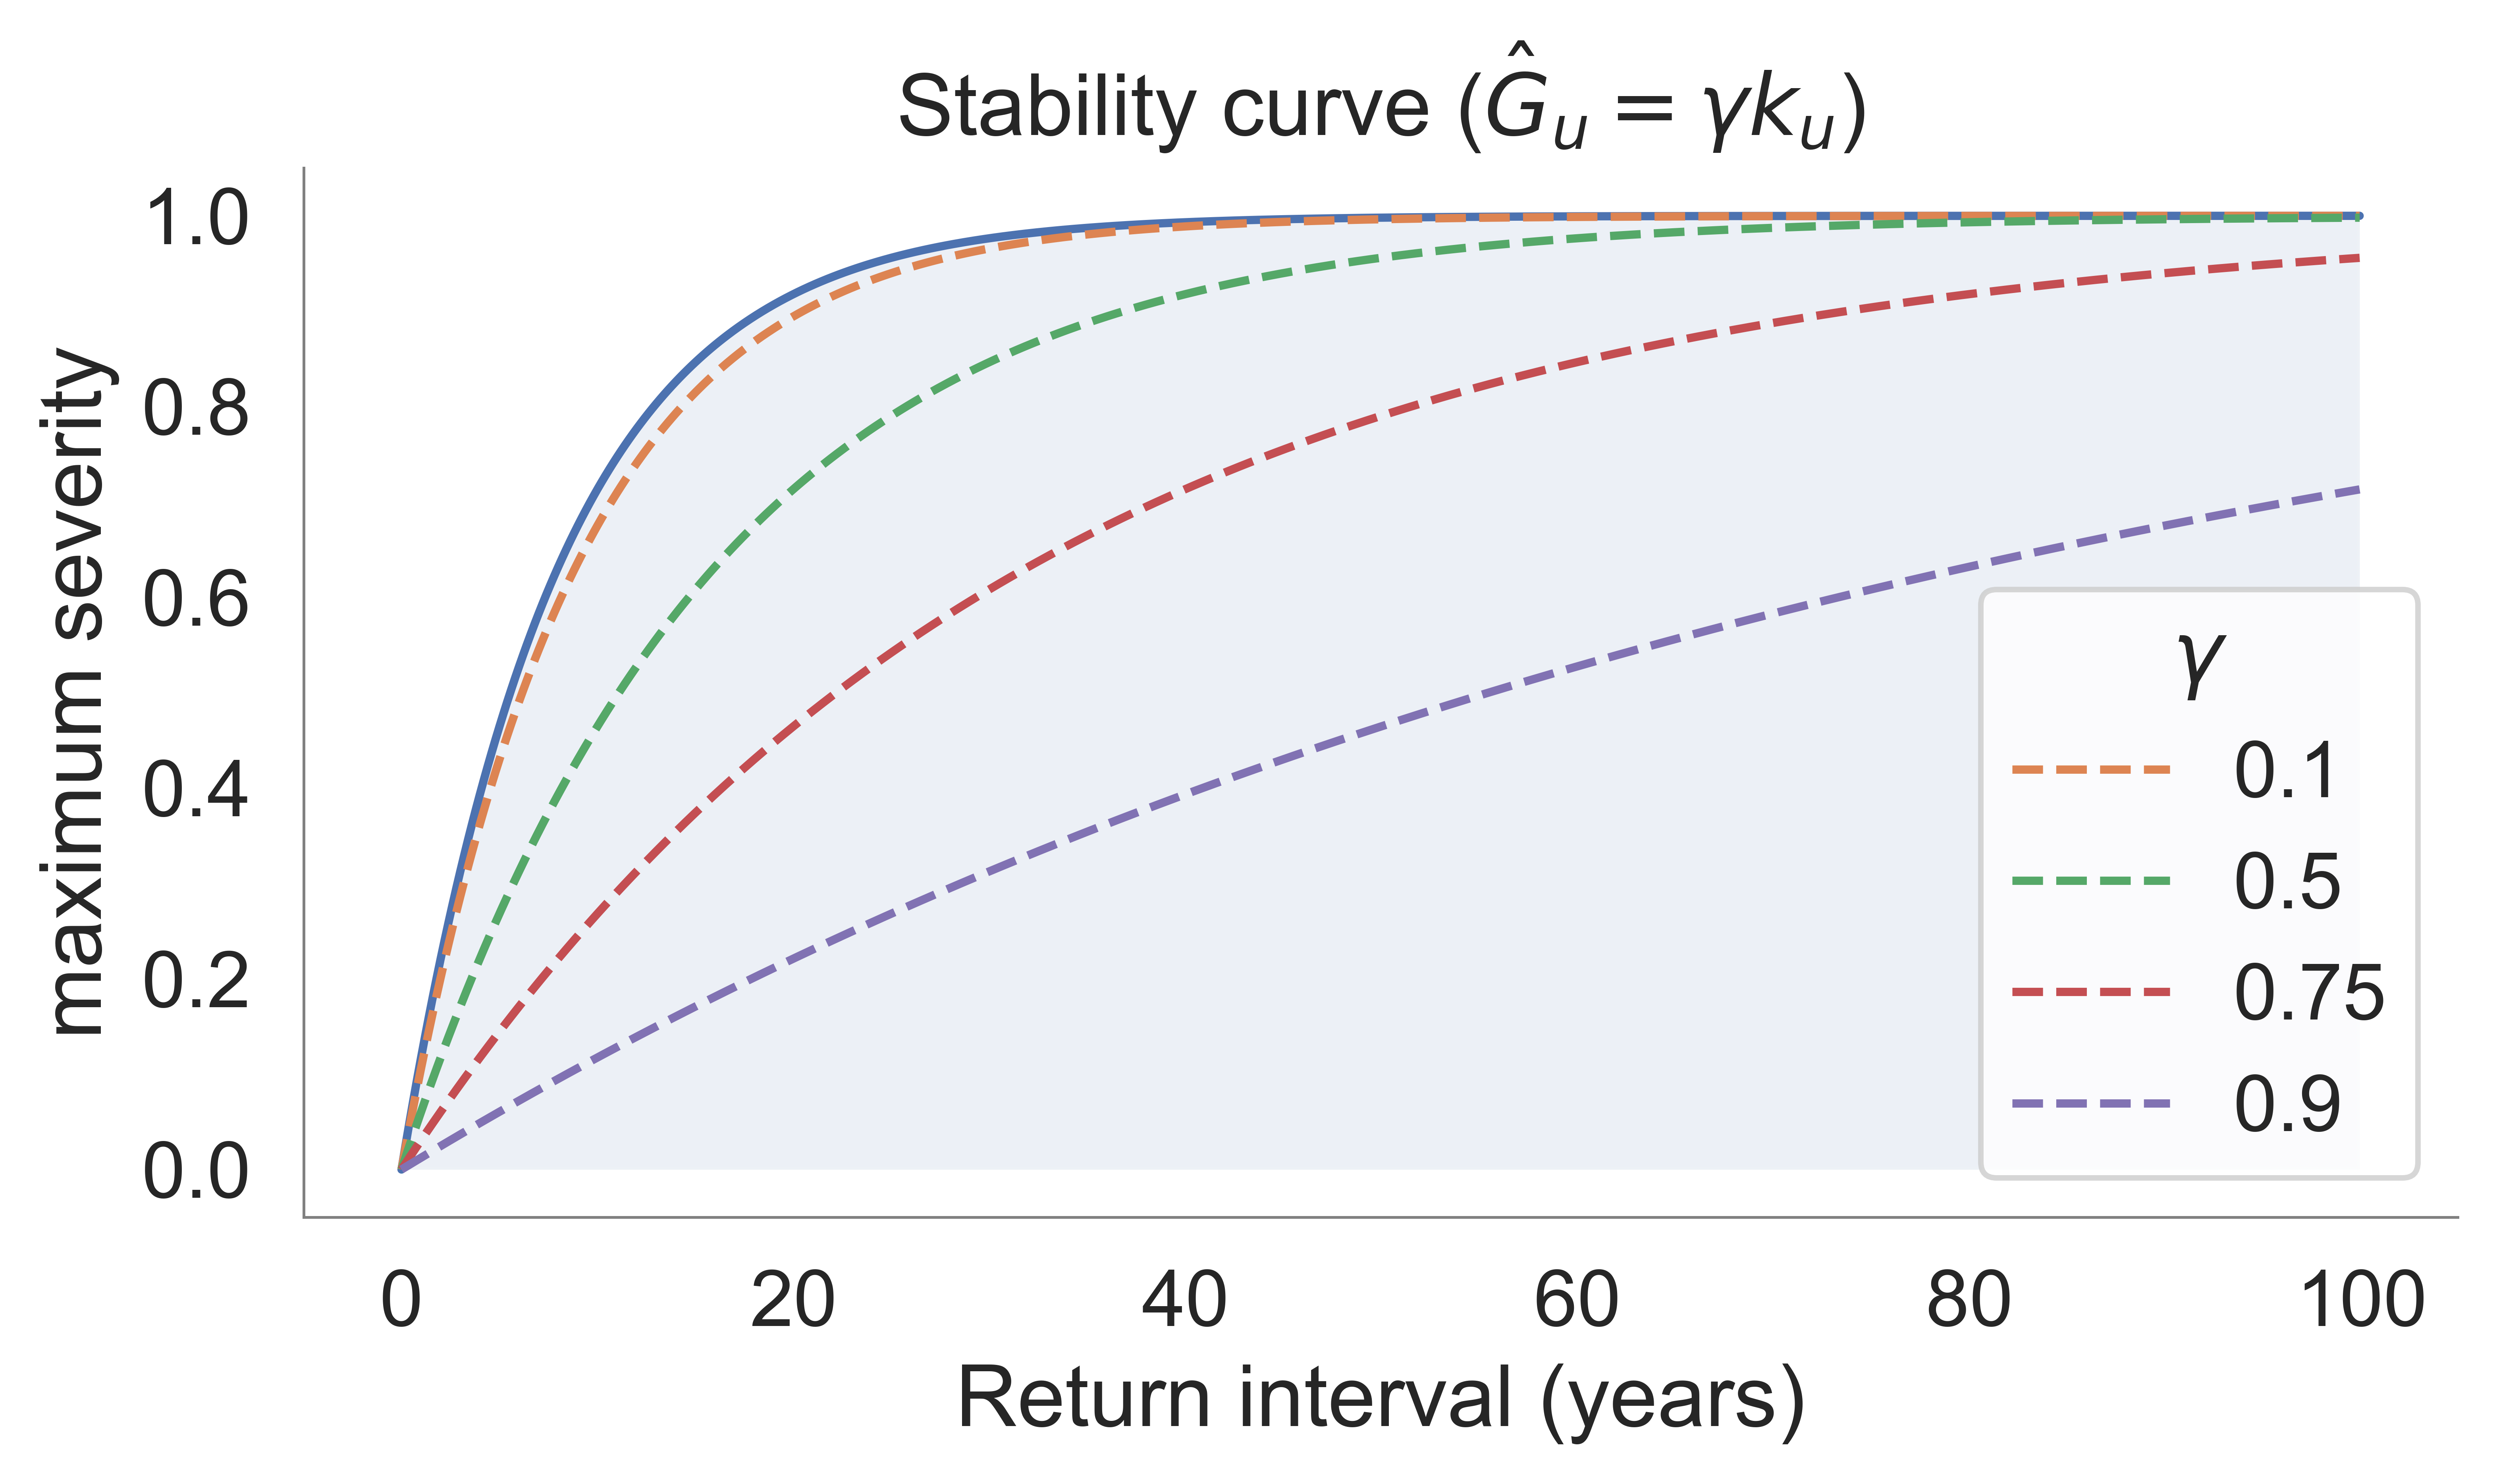
\includegraphics[width=25pc]{../fire_plots/stability.png}
 \caption{ The relationship between $\hat G_u$ and $k_u$ constrains that between $RI$ and severity, and vice versa.}
 \label{fig:stability}
 \end{figure}
   
\subsection{Stability: maximum return interval for a lower canopy}


Equation \ref{hatG_l} can be used to estimate the conditions for which $\hat G_l >0$:

\begin{equation}
\hat{G}_l =
 		k'_l \big( 1 + \frac{1}{r'_l \xi} \log(1-\phi_S) \big) > 0
\end{equation}


\begin{equation}
 		\frac{1}{r'_l \xi} \log(1-\phi_S) > -1
\end{equation}

With some math:

\begin{equation}
 	\xi > - \frac{\log(1-\phi_S)}{r_u S^\beta} \frac{\alpha k_u - r_u S^\beta}{\alpha k_u - r_l S^\beta}
\end{equation}


  \subsection{$\hat G_l$ along a `stability' curve?}

What happens if we move  $G_l$ along the `stability' curve, $\phi_S = 1- e^{-\xi r'_u (1-\gamma)}$?

This expression can be re-witten as:

 $\frac{\log(1 - \phi_S)}{  r'_u \xi  }= -  (1 - \gamma )$


 Substituting into the equations for $r'_l$ and $k'_l$:

\begin{equation}
r'_l= r_l S^\beta   - \alpha k_u \gamma
\end{equation}


\begin{equation}
 k'_l  = k_l  \bigg(1  - \frac{\alpha k_u \gamma} { r_l S^\beta}\bigg)
\end{equation}


Substituting into the Equation for $\hat G_l$:

\begin{equation}
\hat{G}_l =
 		k'_l \big( 1 - \frac{(1 - \gamma) r'_u }{r'_l }  ) \big)
\end{equation}



\begin{equation}
\hat{G}_l =
 		  k_l  \bigg(1  - \frac{\alpha k_u \gamma} { r_l S^\beta}\bigg)
		  \bigg( 1 - \frac{(1 - \gamma) r_u  S^\beta }{(r_l S^\beta   - \alpha k_u \gamma)}   \bigg)
\end{equation}


\begin{equation}
\hat{G}_l =
 		  {k_l}
		  \bigg( 1 - \frac{\alpha k_u \gamma - (1 - \gamma) r_u  S^\beta}{r_l S^\beta }  \bigg)
\end{equation}


\textbf{Take-away}
 The relationship between $\hat G_u$ and $k_u$ also determines how $\hat G_l$ depends on RI and severity.

Above, with $G_l= \gamma k_u$,  $\hat{G}_l$ does not depend on return interval or severity.





\subsection*{Modify ignition probability to decrease with increasing $S$}

Suppose the probability of ignition is: $p = \frac{1-S}{\xi}$.

The effective return time will be: $\xi' = \frac{\xi} { 1- S}$, and the equation for $\hat{G}_u $ becomes:

\begin{equation}
\hat{G}_u =
  k_u \big( 1 + \frac{(1-S)}{r_u S^\beta \xi} \log(1-\phi_S) \big)
\end{equation}

where $\xi$ is now interpretable as the return interval where $S=1$.

 \subsection*{ $G_u$ approaches $k_u$  leading up to each fire. How close does it get?}

The  pre-fire biomass is:

\begin{equation}
  G_{u,max} =  \frac{k_u }{1-\phi_S}   \frac{1- \phi_S - e^{-r'_u \xi} }{1 - e^{-r'_u \xi}}
  \label{G_u_max}
\end{equation}

Expanding, we have:

\begin{equation}
  G_{u,max} =  k_u  \frac{1- \phi_S - e^{-r'_u \xi} }{1  - \phi_S - e^{-r'_u \xi} + \phi_S  e^{-r'_u \xi}}
\end{equation}


Define $x$ as:

\begin{equation}
x = \frac{ \phi_S  e^{-r'_u \xi}}{1- \phi_S - e^{-r'_u \xi}}
\end{equation}

so $ G_{u,max} = k_u /(1+x)$:

\begin{equation}
G_{u,max}  = k_u \frac{1}{1 + \frac{ \phi_S  e^{-r'_u \xi}}{1- \phi_S - e^{-r'_u \xi}}}
\end{equation}


$G_{u,max} \sim k_u$ when $x$ is very small.
Suppose we want $G_{u,max} = \gamma k_u$, where $\gamma$ is close to but less than 1.  Then:


\begin{equation}
 k_u /(1+x) = \gamma k_u
\end{equation}

Rewriting as  $x = 1/\gamma  - 1= C$ (where $C> 0$):

\begin{equation}
 \frac{ \phi_S  e^{-r'_u \xi}}{1- \phi_S - e^{-r'_u \xi}} =  1/\gamma  - 1 = C
\end{equation}

\begin{equation}
{ \phi_S  e^{-r'_u \xi}} = C ({1- \phi_S - e^{-r'_u \xi}} )
\end{equation}

Rearranging gives:

\begin{equation}
 \phi_S   =  \frac{C(1 - e^{-r'_u \xi})}{C  - e^{-r'_u \xi}}
 \label{phi_S_RI}
 \end{equation}

This is an expression for the severity $ \phi_S $ at which $G_u = \gamma k_u$.

Rearranging, the expression for $\xi$ is:


\begin{equation}
\xi   =  \frac{1}{r'_u}\log \frac{C  +\phi_S } {C(1 - \phi_S)}
 \label{RI_phi_S}
 \end{equation}

In the limit that  $G_u = k_u$, $C=0$.
 Equation \ref{phi_S_RI} yields $\phi_S = 0$,  and Equation \ref{RI_phi_S} yields $\xi \rightarrow \inf$.
 This is reassuring.




\section{Soil moisture}

\subsection{How does biomass change with decreasing soil moisture?}

    The derivative of $\hat G_u$ with respect to soil moisture is:
    
    \begin{equation}
    \frac{ d\hat{G}_u }{dS} =
        \begin{cases}
          \frac{-\beta k_u }{r_u \xi} \log(1-\phi_S) S^{-(1+\beta)}
    		& \text{if  } S > \big( - \frac{1}{r_u \xi }\log (1 - \phi_S)\big)^{1/\beta}
    		\\[10pt]
          0 & \text{otherwise}
        \end{cases}
    \end{equation}
    
    
    For the lower canopy, the derivative is:
    
    \begin{equation}
    \frac{ d\hat{G}_l }{dS} =
        \begin{cases}
    	  \frac{\beta  {k_l} }{{r_l} {r_u}} S^{-2 \beta -1}
    \big( {r_u} S^{\beta }(\alpha  {k_u}  - Z) +2 Z \alpha  {k_u}
       \big)
    	  & \text{if  } S > \big( - \frac{1}{r_l \xi }\log (1 - \phi_S)\big)^{1/\beta}
    		\\[10pt]
            \frac{-\beta k_l }{r_l \xi} \log(1-\phi_S) S^{-1-\beta} & \text{otherwise}
        \end{cases}
    \end{equation}
    
    
    where
    
    \begin{equation}
    Z = \frac{\log({1-\phi_S})}{\xi}
    \end{equation}
    
     $\frac{d \hat{G}_l}{dS}$  has a minimum value where
    
      \begin{equation}
      \big( {r_u} S^{\beta }(\alpha  {k_u}  - Z) +2 Z \alpha  {k_u}
       \big) = 0
    \end{equation}
    
    Rearranging:
    
      \begin{equation}
     S^{\beta } = \frac{-2 Z \alpha  {k_u} }{{r_u}(\alpha  {k_u}  - Z)  }
    \end{equation}
    
    Using the definition of $Z$:
    
      \begin{equation}
     S^{\beta } = \frac{-2 {\log({1-\phi_S})} \alpha  {k_u} }{{r_u}(\alpha  {k_u} \xi - {\log({1-\phi_S})})  }
    \end{equation}
    
    The numerator and denominator are both always positive (because $- \log(1-\phi_S) > 0$), so we expect a minima in $\hat G_l$ for $\alpha > 0$.
    
     $\frac{d \hat{G}_l}{dS}$ has a discontinuity at  $ S = \big( - \frac{1}{r_l \xi }\log (1 - \phi_S)\big)^{1/\beta}$, where $G_l$ has a maximum value.
    

\subsection*{Modify ignition probability to decrease with increasing $S$}

Suppose the probability of ignition is: $p = \frac{1-S}{\xi}$.

The effective return time will be: $\xi' = \frac{\xi} { 1- S}$, and the equation for $\hat{G}_u $ becomes:

\begin{equation}
\hat{G}_u =
  k_u \big( 1 + \frac{(1-S)}{r_u S^\beta \xi} \log(1-\phi_S) \big)
\end{equation}

where $\xi$ is now interpretable as the return interval where $S=1$.

 \subsection*{ $G_u$ approaches $k_u$  leading up to each fire. How close does it get?}

The  pre-fire biomass is:

\begin{equation}
  G_{u,max} =  \frac{k_u }{1-\phi_S}   \frac{1- \phi_S - e^{-r'_u \xi} }{1 - e^{-r'_u \xi}}
  \label{G_u_max}
\end{equation}

Expanding, we have:

\begin{equation}
  G_{u,max} =  k_u  \frac{1- \phi_S - e^{-r'_u \xi} }{1  - \phi_S - e^{-r'_u \xi} + \phi_S  e^{-r'_u \xi}}
\end{equation}


Define $x$ as:

\begin{equation}
x = \frac{ \phi_S  e^{-r'_u \xi}}{1- \phi_S - e^{-r'_u \xi}}
\end{equation}

so $ G_{u,max} = k_u /(1+x)$:

\begin{equation}
G_{u,max}  = k_u \frac{1}{1 + \frac{ \phi_S  e^{-r'_u \xi}}{1- \phi_S - e^{-r'_u \xi}}}
\end{equation}


$G_{u,max} \sim k_u$ when $x$ is very small.
Suppose we want $G_{u,max} = \gamma k_u$, where $\gamma$ is close to but less than 1.  Then:


\begin{equation}
 k_u /(1+x) = \gamma k_u
\end{equation}

Rewriting as  $x = 1/\gamma  - 1= C$ (where $C> 0$):

\begin{equation}
 \frac{ \phi_S  e^{-r'_u \xi}}{1- \phi_S - e^{-r'_u \xi}} =  1/\gamma  - 1 = C
\end{equation}

\begin{equation}
{ \phi_S  e^{-r'_u \xi}} = C ({1- \phi_S - e^{-r'_u \xi}} )
\end{equation}

Rearranging gives:

\begin{equation}
 \phi_S   =  \frac{C(1 - e^{-r'_u \xi})}{C  - e^{-r'_u \xi}}
 \label{phi_S_RI}
 \end{equation}

This is an expression for the severity $ \phi_S $ at which $G_u = \gamma k_u$.

Rearranging, the expression for $\xi$ is:


\begin{equation}
\xi   =  \frac{1}{r'_u}\log \frac{C  +\phi_S } {C(1 - \phi_S)}
 \label{RI_phi_S}
 \end{equation}

In the limit that  $G_u = k_u$, $C=0$.
 Equation \ref{phi_S_RI} yields $\phi_S = 0$,  and Equation \ref{RI_phi_S} yields $\xi \rightarrow \inf$.
 This is reassuring.



\section{Estimating parameters}
\subsection{Estimating growth rates from timescales}

Estimate the growth rates from the times for an isolated canopy to grow from $a k_u$ to $b k_u$, where $a$ and $b$ are constants less than 1.
Substituting into the logistic equation solution (with $ G_uo = a k_u$):

\begin{equation}
    b k_u = \frac{k_u  a k_u }{ a k_u +(k_u- a k_u) e^{-r_u \tau}}
\end{equation}

where $\tau$ is the timescale to mature.
\begin{equation}
    b ({ a k_u +(k_u- a k_u) e^{-r_u \tau}) ={ a k_u }}
\end{equation}

\begin{equation}
    b ({ a  +(1- a ) e^{-r'_u t}) ={ a  }}
\end{equation}

\begin{equation}
r_u =   - 1/ \tau \log \big(\frac{a (1-b) }{(1- a )}\big)
\end{equation}


With $a$ = 0.1 and $b$ = 0.9, then $r_u \approx 4.5/ \tau$.

Estimate, growth rates from timescale to mature:

\begin{itemize}
\item conifer : $\tau$=30, $r=0.15$
\item shrubs : $\tau$=10, $r=0.45$
\item meadow : $\tau$=3, $r=1.50$
\item grassland : $\tau$=3, $r=1.50$
\end{itemize}


\section{Non-dimensionalize}

The equations for the upper and lower canopies:

\begin{equation*}
	 \frac{d G_u}{dt} =
	 r_u S^\beta G_u \bigg(1-\frac{G_u}{k_u}\bigg)
\end{equation*}


\begin{equation*}
	 \frac{d G_l}{dt} = r_l S^\beta G_l \bigg(1-\frac{G_l}{k_l}\bigg) - \alpha G_l G_u
\end{equation*}

Non-dimensionalize the upper canopy:

\begin{equation*}
    \frac{d G_u}{dt} =
     \frac{r_u S^\beta}{r_u S^\beta} \frac{G_u}{dt} =
  	{r_u S^\beta} \frac{G_u}{d(r_u S^\beta t)} =
	r_u S^\beta \frac{G_u}{d \tau}
\end{equation*}

where $\tau = r_u S^\beta t$.  Simplifying:

\begin{equation*}
    \frac{d G_u}{d\tau} =
    G_u \bigg(1-\frac{G_u}{k_u}\bigg)
\end{equation*}


Let  $g_u = G_u/k_u$, or   $G_u =   k_u g_u$.  Then:

\begin{equation*}
  \frac{d   g_u}{d\tau} =
	 g_u \bigg(1 -  g_u \bigg)
\end{equation*}

Moving on to the lower canopy.  Substituting $\tau$ for $t$:

\begin{equation*}
	 r_u S^\beta \frac{d G_l}{d \tau } = r_l S^\beta G_l \bigg(1-\frac{G_l}{k_l}\bigg) - \alpha G_l G_u
\end{equation*}

Let  $g_l = G_l/k_l$, or   $G_l =   k_l g_l$.  Then:

\begin{equation*}
r_u   S^\beta \frac{d g_l}{d \tau } = r_l S^\beta k_l g_l \big(1-g_l \big) - \alpha g_l k_l g_u k_u
\end{equation*}

\begin{equation*}
 \frac{d g_l}{d \tau } =\frac{ r_l}{r_u }  g_l \big(1-g_l \big) - \frac{\alpha k_u}{r_u  S^\beta}  g_l g_u
\end{equation*}

So the dimensionless groups are $r_l/r_u$ and $\alpha k_u / S_\beta r_u$, which are a generalized growth rate and competition, respectively.  The rescaled time also need to be factored in:  $\tau = r_u S^\beta t$


%%. 
We have several fixed parameters:  $k_u = 20$, $r_u = 0.25$, $S=0.21$.

$\alpha$ ranges from 0 (no competition) to 0.1,
$\beta$ ranges from 0 (no soil moisture feedback) to 1, $S^\beta$ ranges from 1  to 0.21

let  $r = r_l/r_u$ and $\phi =  \alpha k_u / S_\beta r_u$,

if $r_l$ ranges from 0.25 to 2.5,  $r$ ranges from 1 to 10.


\section{Code notes}

\code{all\_params()} returns the default parameters, which are overwritten when the RCSR class is initialized. 
The only was to change the RCSR parameters is to reinitialize!  





%  \subsection*{Lower canopy equilibrium}
%
%As an alternative approach, what if the lower canopy is in dynamic equilibrium with the upper canopy?
%
%The lower canopy biomass is constant ($\frac{d G_l}{dt}  = 0$) if:
%
%\begin{equation}
% r_l S^\beta G_l \bigg(1-\frac{G_l}{k_l}\bigg) = \alpha G_{u,max} G_l
%\end{equation}
%
%
%Solving for $G_l$:
%
%\begin{equation}
%G_{l,eq}   = k_l\bigg(1 - \frac{ \alpha G_{u,max} }{ r_l S^\beta}\bigg)
%\label{G_l_eq}
%\end{equation}
%
%where $G_{l,eq} $ denotes the equilibrium value for $G_{l} $.
%
%From Equation \ref{G_uo}:
%
%\begin{equation}
%  G_{u,max} = \frac{ k_u}{(1-\phi_S)} \   \frac{1- \phi_S - e^{-r'_u \xi} }{1 - e^{-r'_u \xi}}
%\end{equation}
%
%Substituting, the equation is messy:
%
%\begin{equation}
%G_{l,eq}   = k_l\bigg(1 - \frac{ \alpha  k_u }{ r_l S^\beta}   \frac{(1- \phi_S - e^{-r'_u \xi}) }{(1-\phi_S)(1 - e^{-r'_u \xi)}}   \bigg)
%\end{equation}
%
%If $G_{l,eq}> 0 $, we expect the lower canopy biomass to approach this value in advance of each fire.
%However, if $G_{l,eq}= 0 $, lower canopy biomass may still be present because the system is out of equilibrium!
%
%Estimate a stability boundary as:
%
%
%\begin{equation}
%\frac{\alpha G_{u,max}}{r_l S^\beta} < 1
%\end{equation}
%
%Substituting for $G_{u,max}$:
%
%\begin{equation}
%\frac{\alpha }{r_l S^\beta} \frac{ k_u}{(1-\phi_S)} \   \frac{1- \phi_S - e^{-r'_u \xi} }{1 - e^{-r'_u \xi}} < 1
%\end{equation}
%
%And solving for severity as a function for $\xi$:
%
%
%\begin{equation}
%\phi_S < 1 - \frac{\alpha k_u e^{-r'_u \xi }}{\alpha k_u - r_l S^\beta (1- e^{-r'_u \xi })}
%\end{equation}



\newpage
\bibliographystyle{IEEEtranN}
\bibliographystyle{plain}
\bibliography{references}
\end{document}
